\documentclass{article}
\usepackage[utf8]{inputenc}
\usepackage{amsmath}
\usepackage{graphicx,float}

\title{Synthesis}
\author{Alex Booth\\ a.booth9@edu.salford.ac.uk}
\date{October 2022}

\begin{document}

\maketitle
\section{Abstract}
    \textit{Here goes the abstract}
\section{Introduction}
    Musical instruments have been part of human culture and craft since prehistory, playing a part in both written and verbal art, ceremony and celebration \cite{rault}.
    This report describes an attempted recreation using digital synthesis of two acoustic musical instruments from the western European musical tradition: A Mandolin and a flute.
    Acoustic musical instruments use an excited physical component to generate waves which are manipulated and shaped by the body or construction of the musical instrument. % CITE
    The generation of these waves, and their manipulation by the body of the musical instrument can be modelled using a series of oscillators, filters and modulators.
    Audio synthesis using analog circuitry was explored as soon as simple oscillators were readily available. Leading to instruments such as the theremin.  % WHEN?
    In order to emulate the sound of musical instruments, first we must understand the mathematical nature of sound as a signal.

    FM and additive synthesis methods are explored in this report.

\section{Theory}
    \subsection{Signal processing, generation and analysis}
        Any periodic continuous signal can be broken down into an infinite sum of weighted sines and cosines \cite{weisstein2004fourier}.
        A more generalised application of the Fourier series can be found in the Fourier transform, which in continuous time takes the form:
        \begin{equation}
            X(\omega) = \int_{-\infty}^{+\infty}x(t)e^{-j\omega t}dt
        \end{equation}
        However, as digital audio works in the discrete time domain, the integrals can be represented as sums and the Fourier transform becomes:
        \begin{equation}
            X(\omega) = \sum_{-\infty}^{+\infty}x[n]e^{-j\omega t}dt
        \end{equation}
        In the 1960s, J.W. Cooley and John Tukey developed an algorithm to efficiently compute the discrete Fourier transform \cite{cooley1965algorithm}.
        This, and other discrete-time Fourier transform algorithms became known as the fast Fourier transform(s) (FFT).
        MATLAB's in-built FFT function uses a more modern FFT algorithm from the the FFTW library \cite{frigo1998fftw}.
        Using a Fourier transform, a complex sound can be broken down into it's frequency components.
        This allows the fundamental frequency and harmonics of the played note to be identified, due they will be the most prominent components of the frequency spectrum.
        However, the Fourier transform does not only show harmonic frequency content of a signal, it shows all frequency content of a signal.
        As such, any noise or other anharmonic frequency component, musical or not, will be shown on the transform.
        The simple inclusion of an observed frequency component may or may not be constructive to emulating the original played note.
        \\
        Early musical synthesizers were constructed to facilitate additive synthesis techniques.
        This is where a series of oscillators generate basic waveforms such as sines, sawtooth and pulse waves; a sawtooth wave can be seen in Figure \ref{sawtooth}.
        \begin{figure}[h]
            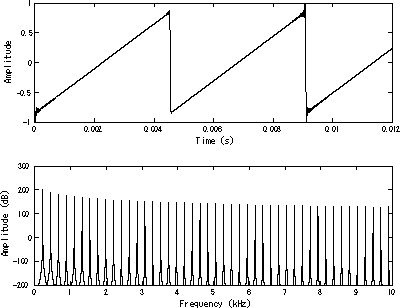
\includegraphics[scale=0.6]{images/Sawtooth.png}%
            \centering
            \caption{Waveform and frequency response of a sawtooth wave.}\cite{kraft2017lp}
            \label{sawtooth}
        \end{figure}
        \\
        These oscillators may be used to generate sound, or used as modulators to other oscillators's outputs.
        Different waveforms generated by these oscillators have different harmonic content.
        For example: in Figure \ref{sawtooth} a sawtooth wave is shown as having many harmonics in the frequency domain plot.
        In fact, a sawtooth wave contains all harmonics, both even and odd, of a fundamental tone \cite{roederer1995physics}.
        In the 1970s, FM synthesis was beginning to take form as a method of musical instrument emulation. Chowning's work outlined specific FM techniques for the emulation of various instruments \cite{chowning1973synthesis}.
        
    \subsection{Musical instruments}

\section{Methodology}
    \subsection{Analysis}
        All code written for this report was executed in MATLAB.
        First, the sample values and sampling rates of the recordings were imported into MATLAB as a vector and constant, respectively.
        Using the sampling rate and total number of samples, a vector of time data was created.
        This allowed the sample values to be plotted against time, as seen in Figure \ref{timeDomainMando}.
        \begin{figure}[h]
            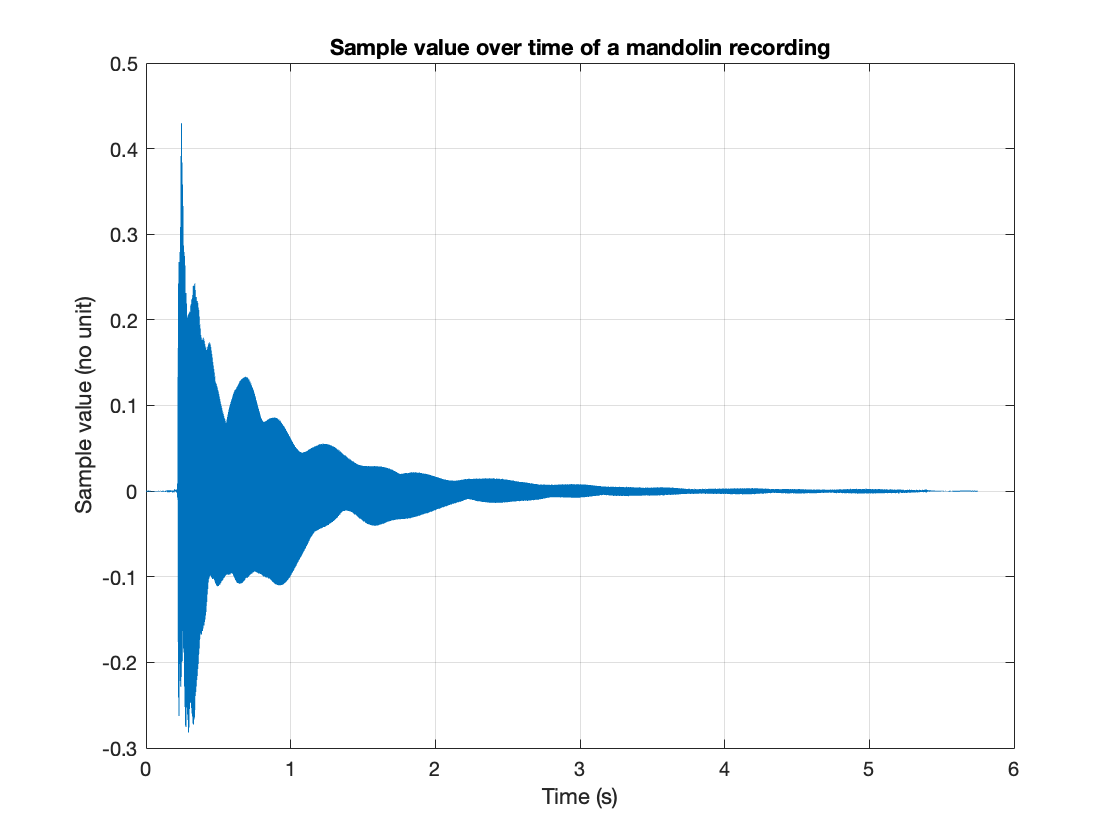
\includegraphics[scale=0.25]{images/timeDomain.png}%
            \centering
            \caption{Mandolin sample value over time.}
            \label{timeDomainMando}
        \end{figure}
        \\
        Next, analysis of the signal in the frequency domain was performed.
        Using MATLAB's in-built FFT function, a frequency domain plot of the signal, averaged over time, was plotted.
        This data was supplemented with another frequency domain plot using \texttt{pwelch()}, a function that uses the Welch algorithm to obtain power spectral density as a function of frequency, instead of sample magnitude \cite{solomon1991psd}.
        A plot of the frequency and phase responses generated by \texttt{pwelch} are shown in Figure \ref{welchMando}.
        \begin{figure}[h]
            
\includegraphics[scale=0.25]{images/placeholder.png}%
            \centering
            \caption{Mandolin sample value over time.}
            \label{welchMando}
        \end{figure}
        The frequency amplitude information gathered from the Fourier transform and Welch power spectral density estimate is averaged over the entire duration of the signal.
        While this information is very useful, it is limited: Much of the frequency content of a signal varies in time, and this time-varying nature of the frequency response contributes greatly to the 
        To see the amplitudes of each frequency component as a function of time, a spectrogram was used.
        MATLAB's \texttt{spectrogram()} function has a high degree of operability and can take many arguments.
        The function works using a 
        Used as a standalone function, it gives the user a two dimensional graph of frequency versus time, with frequency amplitude as a third, coloured dimension.
        There is a trade-off between resolution in the frequency and time domains when using this spectrogram function.
        Higher resolution in the time domain allows for a more visually understandable spectrogram when using a waterfall plot.
        If a high frequency-domain resolution is used, a waterfall plot becomes cluttered and hard to read, as shown 
        Using a hamming window with length $n = 2560$, a 2650-point spectrogram was computed and plotted on a waterfall graph, shown in Figure \ref{specWaterfallMando1}.
        \begin{figure}[h]
            
\includegraphics[scale=0.25]{images/placeholder.png}%
            \centering
            \caption{Mandolin sample value over time.}
            \label{specMando1}
        \end{figure}
        \begin{figure}[h]
            
\includegraphics[scale=0.25]{images/placeholder.png}%
            \centering
            \caption{Mandolin sample value over time.}
            \label{specWaterfallMando1}
        \end{figure}


        



    \subsection{Synthesis}
        Additive synthesis follows the intuition found in Fourier analysis: Any continuous signal is a sum of an infinite number of sine waves.
        Thus, it should be possible to recreate any given signal by breaking it down into it's frequency components, and reproducing these frequency components as sinusoids weighted according to the frequency domain of the analysed signal.
        A programmatic approach was taken in MATLAB: A fourier transform of the recorded signal would return a set of data that may be parsed to find the frequencies of the dominant harmonics of the Mandolin.
        This was implemented by feeding the result of the fourier transform into MATLAB's \texttt{findpeaks()} function, which allows the user to define arguments as to the minimum height and prominence of maxima within a set of data, these maxima would be the harmonics.
        Using \texttt{findpeaks()} required some trial and error adjusting function arguments to avoid less useful peaks within the Fourier transform.
        The found frequencies and their amplitudes will then be substituted into a looping summation of generic sine wave formulae, to produce the output: a complex signal with a similar frequency response to the input; importantly with the same harmonics.
        This formula is shown in Eq.\ref{sineFormula}.
        \begin{equation}
            y[x] = \sum_{n=1}^{N} A_n \sin{2 \pi f_n t}, \text{ where: } n = \text{harmonic number}
            \label{sineFormula}
        \end{equation}

        
        Whilst the spectrograms shown in Figures \ref{specMando1} and \ref{specWaterfallMando1} were useful in illustrating and conveying the amplitude envelopes of a large amount of frequencies across the recording's spectrum, the additive synthesis method chosen chooses to reproduce only a specific few of the harmonic components of the recorded signal.
        Thus, a new spectrogram function will have to be computed targeting these frequency components.
\section{Discussion and Conclusions}
\section{Appendix}
\subsection{Code}



\bibliographystyle{IEEEtran}
\bibliography{theBib.bib}

\end{document}


